Исходные данные

Прокатный цех однопролетный, пролетом 30~м, оборудован двумя мостовыми кранами грузоподъемностью $Q=32/5$~т тяжелого режима работы. Группа режима~8К. Длина здания 120~м, отметка головок рельса 9,4~м. Здание отапливаемое.

Выбрана система с шагом поперечных рам 6~м, с жестким сопряжением ригеля с колонной. Схема поперечной рамы показана на рис.\ref{shrama}
\begin{figure}
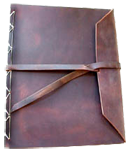
\includegraphics{007.png}
\caption{Схема поперечной рамы однопролетного здания}\label{shrama}
\end{figure}

Вертикальные размеры:

$$H_2\braw(H_k +100)+f=2750+100+350=3200\, \text{мм;}$$
Принимаем $H_2=3200$ мм:
$$H_0=H_1+H_2=9200+3200=12400\,\text{мм.}$$
При высоте подкрановой балки с рельсом, равной 1/8 ее пролета, 
$H_\ruin{в}=(h_{\text{б}}+h_{\text{р}})+H_2=600+200+3200=4000$ мм. 
При заглублении базы колонны на 600 мм ниже пола 
$H_\ruin{н}=H_0-H_\ruin{в}+600=12400-4000+600=9000$ мм. Полная высота колонн 
$H=H_\ruin{в}+H_\ruin{н}=13000$ мм; $H_\ruin{ф}=3150$ мм.

Горизонтальные размеры назначаются следующим образом. В верхней части колонн устраивается проход для осмотра крановых путей, привязка $a=500$ мм, высота сечения верхней части колонны $h_\ruin{в}=700>H_\ruin{в}/12=4000/12=333$ мм. В пределах высоты фермы высоту сечения колонны назначаем $h_\ruin{в}=700$ мм; $l_1\braw B_1+(H_\ruin{в}-a)+75=300+(700-500)+75+450=1025$ мм. Назначаем $l_1=1250$ мм (кратно 250 мм); $h_\ruin{н}=l_1+a=1250+500=1750$ мм. Пролет мостового крана 
$L_\ruin{к}=l-2l_1=30000-2\cdot1250=27500$ мм.

Сечение верхней части колонны назначаем сплошностенчатым двутавровым, нижней --- сквозным.

